\begin{frame}[allowframebreaks]{Transposed Convolution: How It Works}
\begin{figure}
\centering
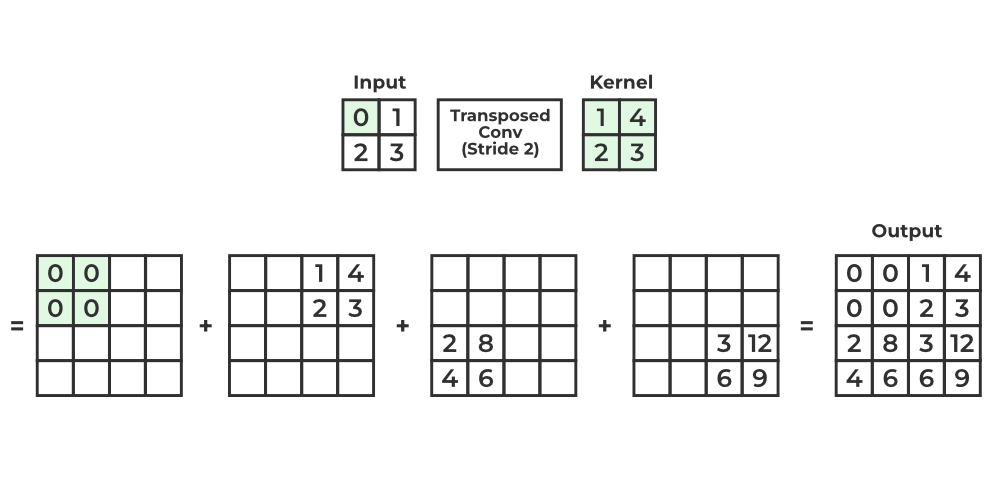
\includegraphics[width=1.0\textwidth,height=1.0\textheight,keepaspectratio]{images/segmentation/TConv.png}
\end{figure}

\framebreak

\begin{figure}
\centering
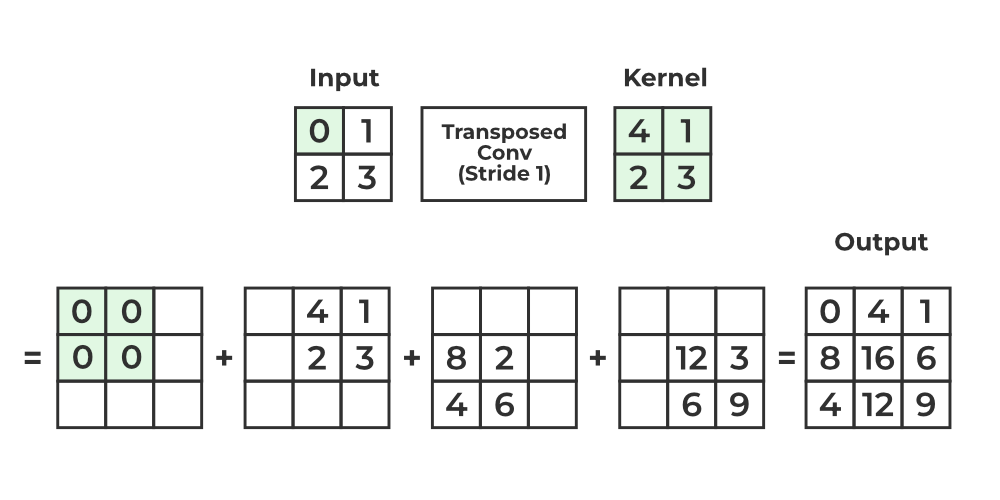
\includegraphics[width=1.0\textwidth,height=1.0\textheight,keepaspectratio]{images/segmentation/TConv2.png}
\end{figure}
\end{frame}

\begin{frame}{Mathematical Definition: Transposed Convolution}
The output \( O(x, y) \) of a transposed convolution is computed as:

\[
O(x, y) = \sum_{i,j} I(i, j) \cdot K(x - i \cdot s, y - j \cdot s)
\]

where:
\begin{itemize}
    \item \( O(x, y) \) is the output at position \( (x, y) \),
    \item \( I(i, j) \) is the input value at \( (i, j) \),
    \item \( K(x', y') \) is the kernel value at \( (x', y') \),
    \item \( s \) is the stride.
\end{itemize}
\end{frame}

\begin{frame}{Transposed Convolution Output Size Formula}

\small
\begin{equation}
\begin{aligned}
H_{\text{out}} &= (H_{\text{in}} - 1) \times \texttt{stride}[0] - 2 \times \texttt{padding}[0] \\
&\quad + \texttt{dilation}[0] \times (\texttt{kernel\_size}[0] - 1) \\
&\quad + \texttt{output\_padding}[0] + 1
\end{aligned}
\end{equation}

\begin{equation}
\begin{aligned}
W_{\text{out}} &= (W_{\text{in}} - 1) \times \texttt{stride}[1] - 2 \times \texttt{padding}[1] \\
&\quad + \texttt{dilation}[1] \times (\texttt{kernel\_size}[1] - 1) \\
&\quad + \texttt{output\_padding}[1] + 1
\end{aligned}
\end{equation}

\vspace{1em}
where:
\begin{itemize}
    \item \( H_{\text{out}}, W_{\text{out}} \) - Output height and width.
    \item \( H_{\text{in}}, W_{\text{in}} \) - Input height and width.
    \item Stride - Step size of the filter movement.
    \item Padding - Number of pixels added around the input.
    \item Dilation - Spacing between kernel elements.
    \item Kernel size - Size of the convolution filter.
    \item Output padding - Additional padding applied to the output.
\end{itemize}
\end{frame}
